\uextra{Apéndice}{Manual de Usuario de NodeLand}
\label{apx:user-manual}

\section*{Introducción a NodeLand}

\textbf{NodeLand} es un lenguaje de programación visual diseñado específicamente para fomentar el desarrollo del pensamiento computacional en niños y jóvenes de 8 a 16 años.

A diferencia de otros lenguajes visuales que se basan en apilar bloques de arriba hacia abajo (flujo de control), NodeLand funciona bajo el paradigma de flujos de datos (dataflow). Aquí, la programación consiste en conectar nodos mediante cables o arcos, dibujando literalmente el camino que recorre la información \textbf{desde que entra hasta que se transforma en un resultado}.

\subsection*{Características Principales}

\begin{itemize}
    \item \textbf{Ejecución Asíncrona y Concurrente:} Los nodos de NodeLand se activan de forma automática tan pronto como reciben información. Esto permite que múltiples caminos de tu programa se ejecuten al mismo tiempo de forma natural.
    \item \textbf{Tipado Visual:} Los distintos tipos de datos (números, textos, verdadero/falso, listas) se identifican rápidamente mediante formas geométricas y colores en sus puertos de conexión, evitando errores.
    \item \textbf{Integración con Hardware:} Permite delegar tareas o conectar tu flujo de datos con placas físicas externas, como la micro:bit (vía Bluetooth o Serial), integrando el mundo digital con el físico.
    \item \textbf{Módulo de Desafíos:} Incluye un mapa de retos gamificados, que te enseñan paso a paso cómo dominar los nodos limitando las herramientas para evitar sobrecargas de información.
\end{itemize}

\section*{Primeros Pasos en el Entorno}

\subsection*{Descripción del Editor}

\begin{figure}[H]
    \centering
    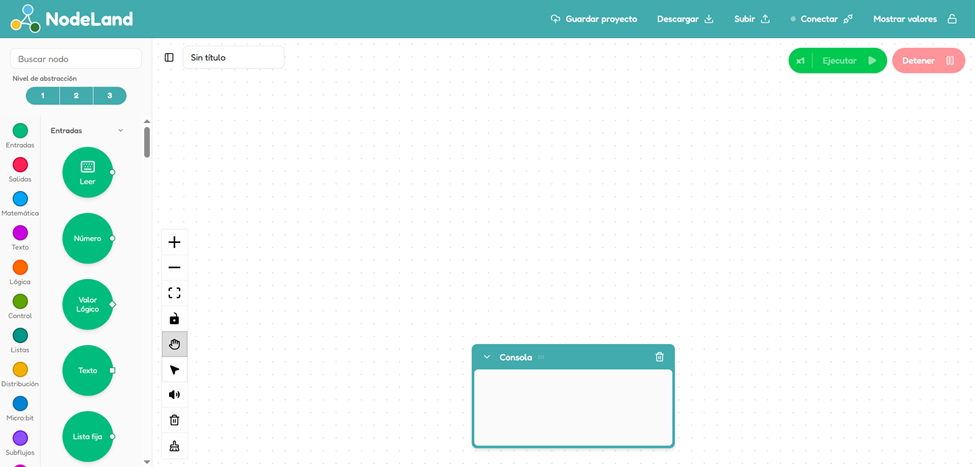
\includegraphics[width=\textwidth]{../images/user-manual/editor.png}
    \caption[Vista del editor]{\normalfont Vista del editor}
\end{figure}

\begin{enumerate}
    \item \textbf{Lienzo de trabajo (Canvas):} Es el área cuadriculada infinita donde construirás tus algoritmos arrastrando y conectando los nodos.
    \item \textbf{Paleta de Nodos:} Situada en el lateral, ofrece un catálogo de herramientas categorizadas por colores y símbolos (Entradas, Procesamiento, Control, Hardware, etc.).
    \item \textbf{Consola de Resultados:} Un área visualmente separada donde el nodo “Escribir” muestra los resultados finales de tus datos.
    \item \textbf{Barra de Herramientas:} En la parte superior encontrarás los botones para Ejecutar (verde) o Detener (rojo) el flujo, además de opciones para Importar o Exportar tus proyectos.
\end{enumerate}

\subsection*{¿Cómo crear un Programa?}

Para programar, solo debes arrastrar nodos al lienzo. Todo nodo tiene “puertos”: los de la izquierda y los de arriba reciben datos y los de la derecha y los de abajo emiten el resultado. Al trazar un arco entre ellos, creas el camino por donde viajará la información.

\begin{figure}[H]
    \centering
    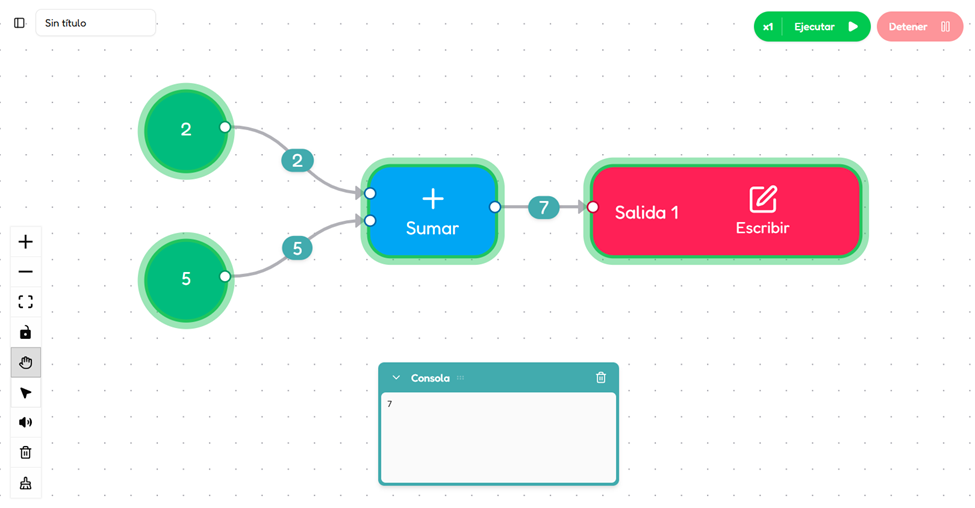
\includegraphics[width=\textwidth]{../images/user-manual/first-program.png}
    \caption[Ejemplo de programa sencillo]{\normalfont Ejemplo de programa sencillo}
\end{figure}

\subsection*{Retroalimentación en Tiempo Real}

Mientras tu programa se ejecuta, NodeLand te avisa visualmente de lo que ocurre:

\begin{itemize}
    \item Borde Gris: El nodo está inactivo, esperando que lleguen datos por su cable.
    \item Borde Azul (animado): ¡Trabajando! El nodo está procesando la información.
    \item Borde Verde: El procesamiento ha finalizado con éxito.
    \item Borde Rojo: Hubo un error (ej: intentaste dividir un número entre 0). Aparecerá un mensaje explicativo.
\end{itemize}

\section*{Programando en NodeLand}

En este apartado exploraremos cómo resolver problemas uniendo nodos. Recuerda que siempre debes presionar el botón verde de “Ejecutar” para que los datos comiencen a fluir por tus cables.

\subsection*{Reto 1. Hola Mundo}

Aprender a unir diferentes trozos de información es el primer paso en la manipulación de datos.
\textbf{Objetivo:} Modificar un texto ingresado agregándole una palabra fija al inicio.
\textbf{Descripción del flujo:}
\begin{enumerate}
    \item Arrastra un nodo Leer (Entrada) al lienzo.
    \item Arrastra un nodo Constante Texto y escribe en él “Hola ”.
    \item Coloca un nodo Concatenar (Texto).
    \item Conecta el cable del nodo Constante Texto a la primera entrada del concatenador, y el cable del nodo Leer a la segunda.
    \item Lleva el cable de salida del Concatenar a un nodo Escribir. Al ejecutar, si ingresas “Ana”, el flujo procesará ambos datos y mostrará “Hola Ana”.
\end{enumerate}

\begin{figure}[H]
    \centering
    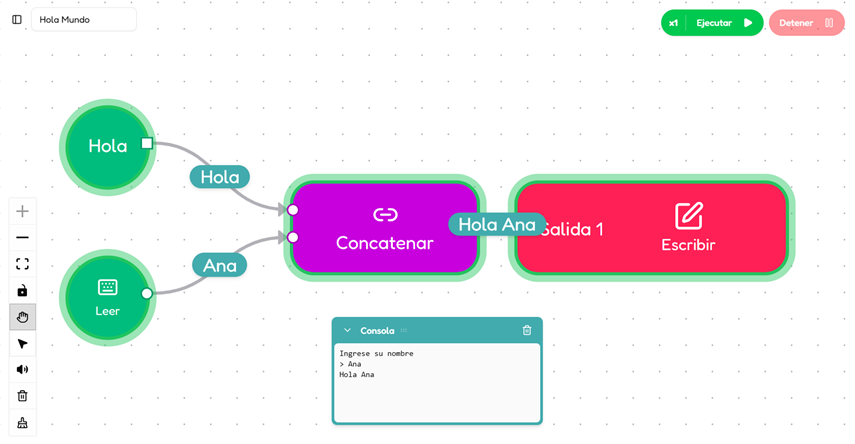
\includegraphics[width=\textwidth]{../images/user-manual/hola-mundo.png}
    \caption[Ejemplo de programa: Hola Mundo]{\normalfont Ejemplo de programa: Hola Mundo}
\end{figure}

\textbf{Propuesta:} Modifica el flujo utilizando un segundo nodo Concatenar para que el resultado final también incluya tu apellido.

\subsection*{Reto 2. Puntos Dobles}

NodeLand hace que las matemáticas sean visuales.
\textbf{Objetivo:} Multiplicar un número que cambie constantemente (una variable) por una constante fija.
\textbf{Descripción del flujo:}
\begin{enumerate}
    \item Imagina que ganaste un “Bonus” en un videojuego. Arrastra un nodo Leer (para tus puntos base) y una Constante Numérica con el valor “2”.
    \item Conecta ambos cables hacia las entradas de un nodo de Multiplicación.
    \item Enlaza la salida al nodo Escribir. ¡Cualquier número que insertes fluirá, se duplicará y saldrá en pantalla!
\end{enumerate}

\begin{figure}[H]
    \centering
    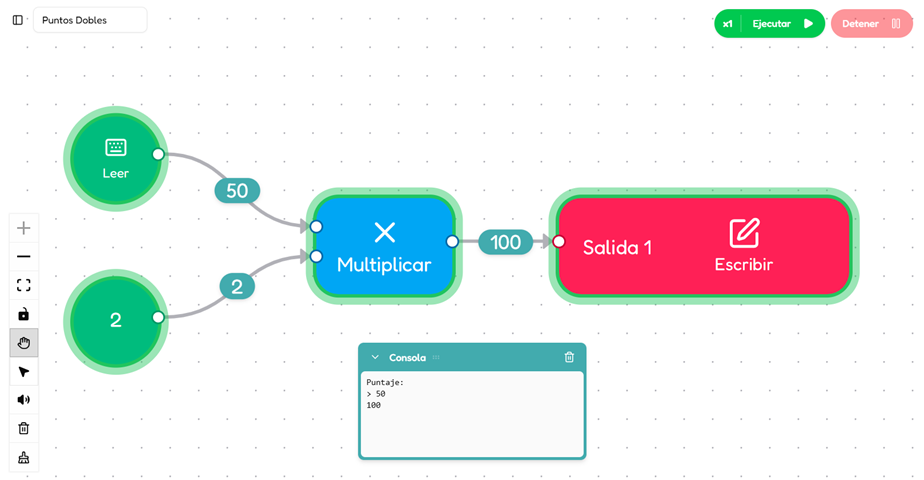
\includegraphics[width=\textwidth]{../images/user-manual/puntos-dobles.png}
    \caption[Ejemplo de programa: Puntos Dobles]{\normalfont Ejemplo de programa: Puntos Dobles}
\end{figure}

\textbf{Propuesta:} Añade un nodo de Suma después de la multiplicación para sumar siempre 10 puntos de regalo al resultado final.

\subsection*{Reto 3. La Puerta Automática}

A veces, los datos deben decidir qué camino tomar.
\textbf{Objetivo:} Enviar datos por rutas diferentes basándose en una condición de Verdadero o Falso.
\textbf{Descripción del flujo:}
\begin{enumerate}
    \item Utiliza un nodo Constante Lógica que actuará como tu interruptor.
    \item Conéctalo al puerto de condición de un nodo Selector.
    \item Crea dos nodos de texto: uno dirá “Abierto” y otro “Cerrado”. Conecta el texto de “Abierto” a la entrada “Verdadero” del selector, y el texto de “Cerrado” a la entrada “Falso” del selector.
    \item Lleva la salida del selector al nodo Escribir. Al cambiar tu interruptor, verás cómo el flujo se enruta por caminos distintos.
\end{enumerate}

\begin{figure}[H]
    \centering
    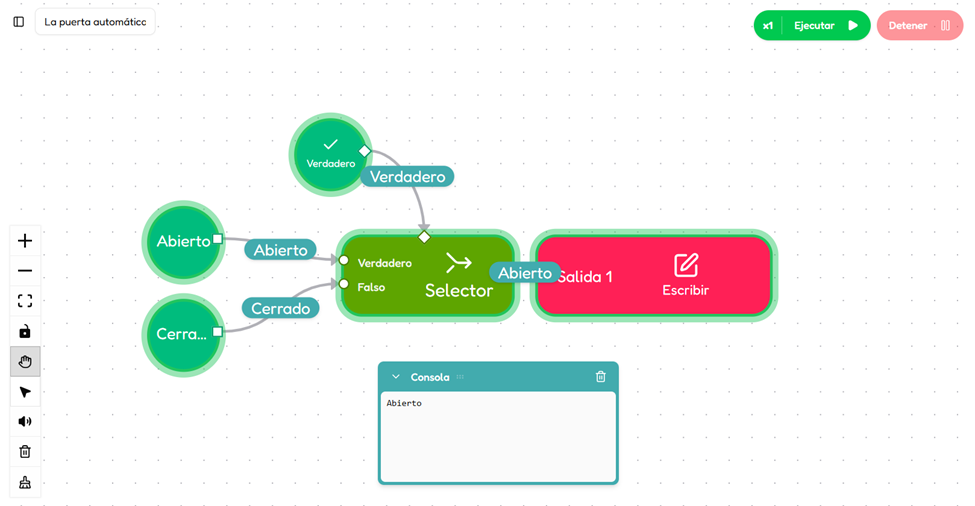
\includegraphics[width=\textwidth]{../images/user-manual/puerta-automatica.png}
    \caption[Ejemplo de programa: La Puerta Automática]{\normalfont Ejemplo de programa: La Puerta Automática}
\end{figure}

\textbf{Propuesta:} Sustituye la constante lógica por un nodo Comparar, para que la puerta diga “Abierto” únicamente si introduces el número “1234”.

\subsection*{Reto 4. Caminos Paralelos}

A diferencia de los lenguajes tradicionales, en NodeLand un dato puede clonarse y hacer dos cosas a la vez.
\textbf{Objetivo:} Entender cómo dividir un cable para ejecutar algoritmos paralelos.
\textbf{Descripción del flujo:}
\begin{enumerate}
    \item Coloca un nodo Constante Numérica con el valor “10”. Haz clic en su puerto de salida y arrastra dos cables distintos.
    \item El primer cable irá directo a la primera entrada de un nodo Suma.
    \item El segundo cable pasará primero por un nodo Multiplicación (multiplicado por 2), y la salida de esto irá a la segunda entrada del nodo Suma. El motor de ejecución de NodeLand mandará el “10” por ambos cables al mismo tiempo. Uno llegará intacto y el otro se volverá “20”.
    \item El nodo de Suma esperará a que lleguen ambos para dar “30” como resultado.
\end{enumerate}

\begin{figure}[H]
    \centering
    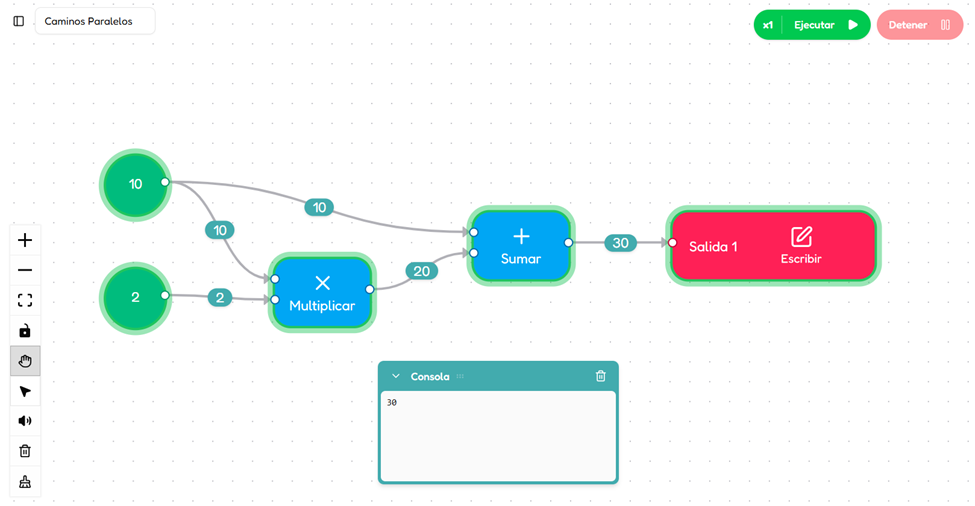
\includegraphics[width=\textwidth]{../images/user-manual/caminos-paralelos.png}
    \caption[Ejemplo de programa: Caminos Paralelos]{\normalfont Ejemplo de programa: Caminos Paralelos}
\end{figure}

\subsection*{Reto 5. Integración Física con Micro:bit}

NodeLand posee un sistema Orquestador que puede repartir el trabajo fuera del navegador.
\textbf{Objetivo:} Usar la tarjeta micro:bit como una fuente activa de datos.
\textbf{Descripción del flujo:}
\begin{enumerate}
    \item En lugar de un nodo “Leer”, busca en tu paleta los nodos de Micro:bit. Arrastra el nodo Leer Botón y conéctalo a un nodo Escribir.
    \item Asegúrate de emparejar tu tarjeta mediante el menú, presionando el ícono del botón (Bluetooth o Serial).
    \item Al ejecutar el programa, el lenguaje enviará instrucciones a tu placa. ¡Cuando presiones el botón A de tu micro:bit, la letra fluirá directamente a través del lienzo en tu pantalla!
\end{enumerate}

\begin{figure}[H]
    \centering
    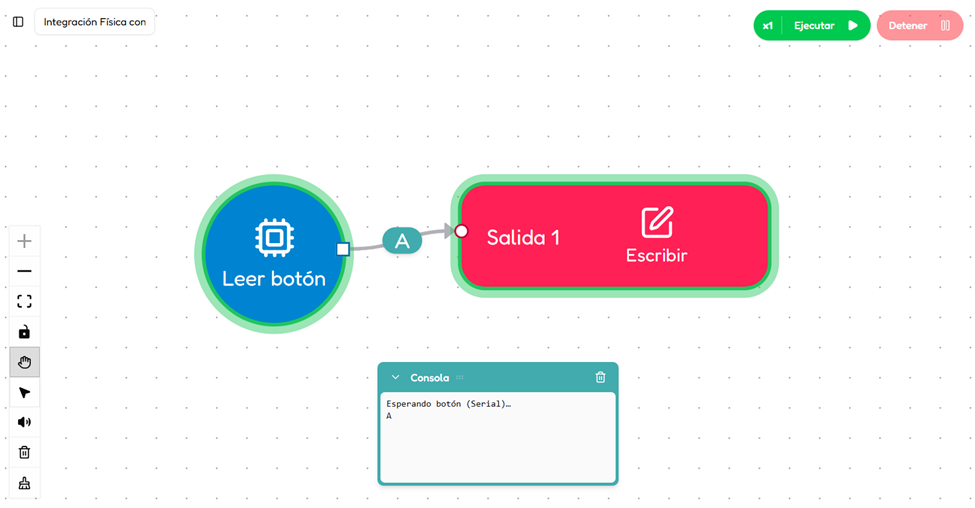
\includegraphics[width=\textwidth]{../images/user-manual/microbit.png}
    \caption[Ejemplo de programa: Integración Física con Micro:bit]{\normalfont Ejemplo de programa: Integración Física con Micro:bit}
\end{figure}

\textbf{Propuesta:} Conecta el resultado del botón a un nodo Condicional, de forma que si presionas el botón “A” la consola escriba el resultado, y si presionas el “B” no pase nada.
